%iffalse
\let\negmedspace\undefined
\let\negthickspace\undefined
\documentclass[journal,12pt,onecolumn]{IEEEtran}
\usepackage{cite}
\usepackage{amsmath,amssymb,amsfonts,amsthm}
\usepackage{algorithmic}
\usepackage{graphicx}
\usepackage{textcomp}
\usepackage{xcolor}
\usepackage{txfonts}
\usepackage{listings}
\usepackage{enumitem}
\usepackage{mathtools}
\usepackage{gensymb}
\usepackage{comment}
\usepackage[breaklinks=true]{hyperref}
\usepackage{tkz-euclide} 
\usepackage{listings}
\usepackage{gvv}                                        
%\def\inputGnumericTable{}                                 
\usepackage[latin1]{inputenc}     
\usepackage{xparse}
\usepackage{color}                                            
\usepackage{array}                                            
\usepackage{longtable}                                       
\usepackage{calc}                                             
\usepackage{multirow}
\usepackage{multicol}
\usepackage{hhline}                                           
\usepackage{ifthen}                                           
\usepackage{lscape}
\usepackage{tabularx}
\usepackage{array}
\usepackage{float}
\newtheorem{theorem}{Theorem}[section]
\newtheorem{problem}{Problem}
\newtheorem{proposition}{Proposition}[section]
\newtheorem{lemma}{Lemma}[section]
\newtheorem{corollary}[theorem]{Corollary}
\newtheorem{example}{Example}[section]
\newtheorem{definition}[problem]{Definition}
\newcommand{\BEQA}{\begin{eqnarray}}
\newcommand{\EEQA}{\end{eqnarray}}
\usepackage{float}

\theoremstyle{remark}
\usepackage{ circuitikz }



\title{GATE-IN-2020}
\author{EE25BTECH11002 - Achat Parth Kalpesh }
\date{}

\begin{document}

\maketitle
\section*{Q.1-Q.5 carry one mark each. }

\begin{enumerate}
\item He is known for his unscrupulous ways. He always sheds \rule{2cm}{0.4pt} tears to deceive people.

\hfill{(GATE IN 2020)}
\begin{enumerate}
\begin{multicols}{4}
\item fox's
\item crocodile's
\item crocodile
\item fox
\end{multicols}
\end{enumerate}

\item Jofra Archer, the England fast bowler, is \rule{2cm}{0.4pt} than accurate.

\hfill{(GATE IN 2020)}
\begin{enumerate}
\begin{multicols}{4}
\item more fast
\item faster
\item less fast
\item more faster
\end{multicols}
\end{enumerate}

\item Select the word that fits the analogy:
\par Build : Building :: Grow : \rule{2cm}{0.4pt}

\hfill{(GATE IN 2020)}
\begin{enumerate}
\item Grown
\item Grew
\item Growth
\item Growed
\end{enumerate}

\item I do not think you know the case well enough to have opinions. Having said that, I agree with your other point.
What does the phrase "having said that" mean in the given text?

\hfill{(GATE IN 2020)}
\begin{enumerate}
\item as opposed to what I have said
\item despite what I have said
\item in addition to what I have said
\item contrary to what I have said
\end{enumerate}

\item Define $\sbrak{x}$ as the greatest integer less than or equal to $x$, for each $x \in \brak{-\infty, \infty}$. If $y = \sbrak{x}$, then area under $y$ for $x \in \sbrak{1,4}$ is \rule{2cm}{0.4pt}.

\hfill{(GATE IN 2020)}
\begin{enumerate}
\begin{multicols}{4}
\item $1$
\item $3$
\item $4$
\item $6$
\end{multicols}
\end{enumerate}

\textbf{Q.6 - Q.10 carry two marks each.}

\item Crowd funding deals with mobilisation of funds for a project from a large number of people, who would be willing to invest smaller amounts through web-based platforms in the project.
\par Based on the above paragraph, which of the following is correct about crowd funding?

\hfill{(GATE IN 2020)}
\begin{enumerate}
\item Funds raised through unwilling contributions on web-based platforms.
\item Funds raised through large contributions on web-based platforms.
\item Funds raised through coerced contributions on web-based platforms.
\item Funds raised through voluntary contributions on web-based platforms.
\end{enumerate}

\item P, Q, R and S are to be uniquely coded using $\alpha$ and $\beta$. If P is coded as $\alpha\alpha$ and Q as $\alpha\beta$, then R and S, respectively, can be coded as \rule{2cm}{0.4pt}

\hfill{(GATE IN 2020)}
\begin{enumerate}
\begin{multicols}{2}
\item $\beta\alpha$ and $\alpha\beta$
\item $\beta\beta$ and $\alpha\alpha$
\item $\alpha\beta$ and $\beta\beta$
\item $\beta\alpha$ and $\beta\beta$
\end{multicols}
\end{enumerate}

\item The sum of the first $n$ terms in the sequence $8, 88, 888, 8888, \dots$ is \rule{2cm}{0.4pt}

\hfill{(GATE IN 2020)}
\begin{enumerate}
\begin{multicols}{2}
\item $\frac{81}{80}\brak{10^n - 1} + \frac{9}{8}n$
\item $\frac{81}{80}\brak{10^n - 1} - \frac{9}{8}n$
\item $\frac{80}{81}\brak{10^n - 1} + \frac{8}{9}n$
\item $\frac{80}{81}\brak{10^n - 1} - \frac{8}{9}n$
\end{multicols}
\end{enumerate}

\item Select the graph that schematically represents BOTH $y = x^m$ and $y = x^{1/m}$ properly in the interval $0 \leq x \leq 1$, for integer values of $m$, where $m > 1$.

\hfill{(GATE IN 2020)}

\begin{enumerate}
\begin{multicols}{2}
\item 
    \begin{figure}[H]
\centering
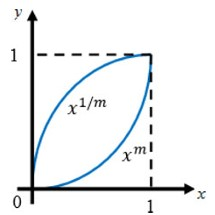
\includegraphics[width=0.7\columnwidth]{figs/q1.jpg}
\caption*{}
\label{fig:q1}
\end{figure}

\item 
   \begin{figure}[H]
\centering
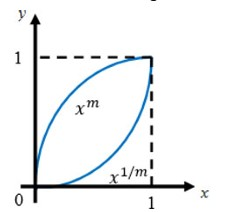
\includegraphics[width=0.7\columnwidth]{figs/q2.jpg}
\caption*{}
\label{fig:q2}
\end{figure}

\item
   \begin{figure}[H]
\centering
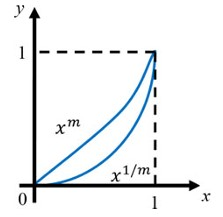
\includegraphics[width=0.7\columnwidth]{figs/q3.jpg}
\caption*{}
\label{fig:q3}
\end{figure}

\item
    \begin{figure}[H]
\centering
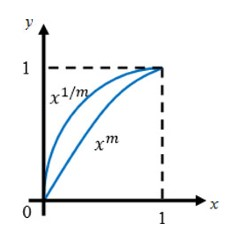
\includegraphics[width=0.7\columnwidth]{figs/q4.jpg}
\caption*{}
\label{fig:q4}
\end{figure}
\end{multicols}
\end{enumerate}

\item The bar graph\figref{fig:q5} shows the data of the students who appeared and passed in an examination for four schools P, Q, R and S. The average of success rates \brak{\text{in percentage}} of these four schools is \rule{2cm}{0.4pt}

\begin{figure}[H]
\centering
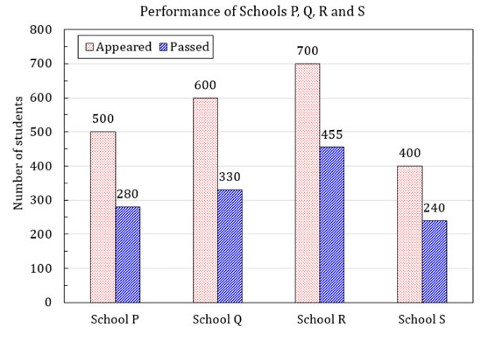
\includegraphics[width=0.7\columnwidth]{figs/q5.jpg}
\caption*{}
\label{fig:q5}
\end{figure}

\hfill{(GATE IN 2020)}
\begin{enumerate}
\begin{multicols}{4}
\item $58.5\,\%$
\item $58.8\,\%$
\item $59.0\,\%$
\item $59.3\,\%$
\end{multicols}
\end{enumerate}

\end{enumerate}

\section*{INSTRUMENTATION ENGINEERING}

\textbf{Q1 - Q25 carry one mark each.}    

\begin{enumerate}

\item The unit vectors along the mutually perpendicular $x, y$ and $z$ axes are $\hat{i}, \hat{j}$ and $\hat{k}$ respectively. Consider the plane $z = 0$ and two vectors $\vec{a}$ and $\vec{b}$ on that plane such that $\vec{a} \neq \alpha \vec{b}$ for any scalar $\alpha$. A vector perpendicular to both $\vec{a}$ and $\vec{b}$ is \rule{2cm}{0.4pt}

\hfill{(GATE IN 2020)}
\begin{enumerate}
\begin{multicols}{4}
\item $\hat{k}$
\item $\hat{i} - \hat{j}$
\item $-\hat{j}$
\item $\hat{i}$
\end{multicols}
\end{enumerate}

\item Consider the recursive equation $X_{n+1} = X_n - h \brak{ F\brak{X_n} - X_n }$, with initial condition $X_0 = 1$ and $h > 0$ being a very small valued scalar. This recursion numerically solves the ordinary differential equation \rule{2cm}{0.4pt}

\hfill{(GATE IN 2020)}
\begin{enumerate}
\begin{multicols}{2}
\item $\dot{X} = -F\brak{X}, X\brak{0} = 1$
\item $\dot{X} = -F\brak{X} + X, X\brak{0} = 1$
\item $\dot{X} = F\brak{X}, X\brak{0} = 1$
\item $\dot{X} = F\brak{X} + X, X\brak{0} = 1$
\end{multicols}
\end{enumerate}

\item A set of linear equations is given in the form $Ax = b$, where $A$ is a $2 \times 4$ matrix with real number entries and $b \neq 0$. Will it be possible to solve for $x$ and obtain a unique solution by multiplying both left and right sides of the equation by $A^T$ \brak{\text{the super script T denotes the transpose}} and inverting the matrix $A^T A$? Answer is \rule{2cm}{0.4pt}

\hfill{(GATE IN 2020)}
\begin{enumerate}
\item Yes, it is always possible to get a unique solution for any $2 \times 4$ matrix $A$.
\item No, it is not possible to get a unique solution for any $2 \times 4$ matrix $A$.
\item Yes, can obtain a unique solution provided the matrix $A^T A$ is well conditioned
\item Yes, can obtain a unique solution provided the matrix $A$ is well conditioned
\end{enumerate}

\item In the circuit shown below,\figref{fig:q6} the safe maximum value for the current I is \rule{2cm}{0.4pt}
\begin{figure}[H]
\centering
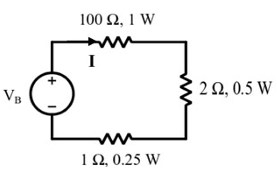
\includegraphics[width=0.4\columnwidth]{figs/q6.jpg}
\caption*{}
\label{fig:q6}
\end{figure}

\hfill{(GATE IN 2020)}
\begin{enumerate}
\begin{multicols}{4}
\item $1.0$ A
\item $0.5$ A
\item $0.1$ A
\item $0.05$ A
\end{multicols}
\end{enumerate}

\item A differentiator has a transfer function whose \rule{2cm}{0.4pt}

\hfill{(GATE IN 2020)}
\begin{enumerate}
\item phase increases linearly with frequency
\item magnitude remains constant
\item magnitude increases linearly with frequency
\item magnitude decreases linearly with frequency
\end{enumerate}

\item A phase lead network has the transfer function $G\brak{s} = \frac{1+0.2s}{1+0.05s}$. The angular frequency at which the maximum phase shift for the network occurs is \rule{2cm}{0.4pt}

\hfill{(GATE IN 2020)}
\begin{enumerate}
\begin{multicols}{4}
\item $10$ rad/s
\item $20$ rad/s
\item $100$ rad/s
\item $200$ rad/s
\end{multicols}
\end{enumerate}

\item If the diodes in the circuit shown\figref{fig:q7} are ideal and the breakdown voltage $V_z$ of the Zener diode is $5$ V, the power dissipated in the $100~\ohm$ resistor \brak{\text{in watts}} is \rule{2cm}{0.4pt}
\begin{figure}[H]
\centering
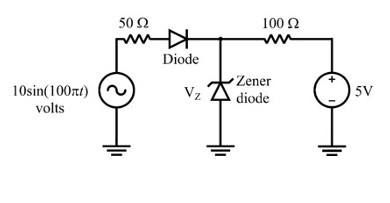
\includegraphics[width=0.5\columnwidth]{figs/q7.jpg}
\caption*{}
\label{fig:q7}
\end{figure}

\hfill{(GATE IN 2020)}
\begin{enumerate}
\begin{multicols}{4}
\item $0$
\item $1$
\item $25/100$
\item $225/100$
\end{multicols}
\end{enumerate}

\item Given $f \brak{A, B, C, D} = \sum m\brak{0, 1, 2, 6, 8, 9, 10, 11} + \sum d\brak{3, 7, 14, 15}$ is a Boolean function, where $m$ represents min-terms and $d$ represents don't-cares. The minimal sum of products expression for $f$ is \rule{2cm}{0.4pt}

\hfill{(GATE IN 2020)}
\begin{enumerate}
\begin{multicols}{2}
\item $f = \bar{A}\bar{B} + C\bar{B}$
\item $f = \bar{B} + C$
\item $f = \bar{D} + A$
\item $f = A\bar{B} + C\bar{D}$
\end{multicols}
\end{enumerate}

\item A Q meter is best suited for the measurement of the \rule{2cm}{0.4pt}

\hfill{(GATE IN 2020)}
\begin{enumerate}
\item Quality factor of a capacitance.
\item Distributed capacitance of a coil.
\item Quality factor of piezoelectric sensor.
\item Turns-ratio of a transformer
\end{enumerate}

\item If $I$ is the current flowing through a Hall effect sensor and $B$ is the magnetic flux density perpendicular to the direction of the current \brak{\text{in the plane of the Hall effect sensor}}, the Hall voltage generated is \rule{2cm}{0.4pt}

\hfill{(GATE IN 2020)}
\begin{enumerate}
\item Directly proportional to $I$ and inversely proportional to $B$
\item Directly proportional to both $I$ and $B$
\item Inversely proportional to both $I$ and $B$
\item Inversely proportional to $I$ and directly proportional to $B$
\end{enumerate}

\item The Boolean expression for the shaded regions as shown in the figure\figref{fig:q8} is \rule{2cm}{0.4pt}
\begin{figure}[H]
\centering
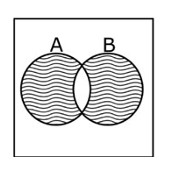
\includegraphics[width=0.3\columnwidth]{figs/q8.jpg}
\caption*{}
\label{fig:q8}
\end{figure}

\hfill{(GATE IN 2020)}
\begin{enumerate}
\begin{multicols}{2}
\item $\brak{A+B}\cdot\brak{\bar{A}+\bar{B}}$
\item $\brak{\bar{A}+B}\cdot\brak{A+\bar{B}}$
\item $\brak{\bar{A}+\bar{B}}\cdot\brak{A+B}$
\item $\brak{A+\bar{B}}\cdot\brak{A+B}$
\end{multicols}
\end{enumerate}

\item The Boolean operation performed by the following circuit\figref{fig:q9} at the output O is \rule{2cm}{0.4pt}
\begin{figure}[H]
\centering
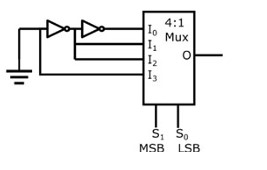
\includegraphics[width=0.4\columnwidth]{figs/q9.jpg}
\caption*{}
\label{fig:q9}
\end{figure}

\hfill{(GATE IN 2020)}
\begin{enumerate}
\begin{multicols}{2}
\item $O = S_1 \oplus S_0$
\item $O = S_1\cdot \overline{S_0}$
\item $O = S_1 + S_0$
\item $O = S_0 \cdot \overline{S_1}$
\end{multicols}
\end{enumerate}

\item Consider the Signal $x\sbrak{n} = \sin\brak{2\pi n} u\sbrak{n}$, where $u\sbrak{n} = \begin{cases} 1 & n = 0,1,2,3, \dots \\ 0 & \text{otherwise} \end{cases}$. The period of this signal $x\sbrak{n}$ is \rule{2cm}{0.4pt}

\hfill{(GATE IN 2020)}
\begin{enumerate}
\begin{multicols}{4}
\item $4$
\item $3$
\item $2$
\item $1$
\end{multicols}
\end{enumerate}

\item The closed loop transfer function of a control system is given by $\frac{C\brak{s}}{R\brak{s}} = \frac{1}{s+1}$. For the input $r\brak{t} = \sin t$, the steady state response $c\brak{t}$ is \rule{2cm}{0.4pt}

\hfill{(GATE IN 2020)}
\begin{enumerate}
\begin{multicols}{2}
\item $1$
\item $\frac{1}{\sqrt{2}} \cos t$
\item $\frac{1}{\sqrt{2}} \sin \brak{t + \frac{\pi}{4}}$
\item $\frac{1}{\sqrt{2}} \sin \brak{t - \frac{\pi}{4}}$
\end{multicols}
\end{enumerate}

\item Let $f\brak{z} = \frac{1}{z+a}, a > 0$. The value of the integral $\oint f\brak{z}dz$ over a circle C with center $\brak{-a, 0}$ and radius $R > 0$ evaluated in the anti-clockwise direction is \rule{2cm}{0.4pt}

\hfill{(GATE IN 2020)}
\begin{enumerate}
\begin{multicols}{4}
\item $0$
\item $2\pi i$
\item $-2\pi i$
\item $4\pi i$
\end{multicols}
\end{enumerate}

\item A player throws a ball at a basket kept at a distance. The probability that the ball falls into the basket in a single attempt is $0.1$. The player attempts to throw the ball twice. Considering each attempt to be independent, the probability that this player puts the ball into the basket only in the second attempt \brak{\text{rounded off to two decimal places}} is \rule{2cm}{0.4pt}

\hfill{(GATE IN 2020)}

\item Assuming ideal opamps, the output voltage at $V_1$ in the figure shown\figref{fig:q10} \brak{\text{in volts}} is \rule{2cm}{0.4pt}
\begin{figure}[H]
\centering
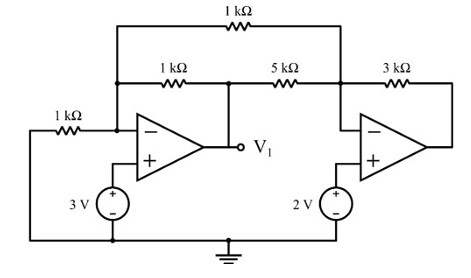
\includegraphics[width=0.6\columnwidth]{figs/q10.jpg}
\caption*{}
\label{fig:q1}
\end{figure}

\hfill{(GATE IN 2020)}

\item Three $400~\ohm$ resistors are connected in delta and powered by a $400$ V \brak{\text{rms}}, $50$ Hz, balanced, symmetrical R-Y-B sequence, three-phase three-wire mains. The rms value of the line current is \rule{2cm}{0.4pt} \brak{\text{in amperes, rounded off to one decimal place}}

\hfill{(GATE IN 2020)}

\item Consider the signal $x\brak{t} = e^{-\abs{t}}$. Let $X\brak{j\omega} = \int_{-\infty}^{\infty} x\brak{t} e^{-j\omega t} dt$ be the Fourier transform of $x\brak{t}$. The value of $X\brak{j0}$ is \rule{2cm}{0.4pt}

\hfill{(GATE IN 2020)}

\item A second order system has closed loop poles located at 
$s = -3 \underset{-}{+} j4$. The time $t$ at which the maximum value of the step response occurs \brak{\text{in seconds, rounded off to two decimal places}} is \rule{2cm}{0.4pt}

\hfill{(GATE IN 2020)}

\item Assume that the opamp in the circuit shown\figref{fig:q11} is ideal. The value of $\frac{V_x}{I_x}$ \brak{\text{in k}\ohm} is \rule{2cm}{0.4pt}
\begin{figure}[H]
\centering
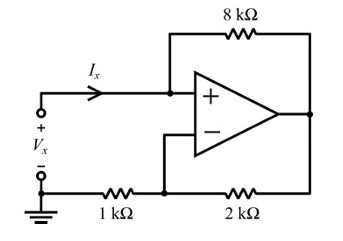
\includegraphics[width=0.4\columnwidth]{figs/q11.jpg}
\caption*{}
\label{fig:q11}
\end{figure}

\hfill{(GATE IN 2020)}

\item A sinusoid of $10$ kHz is sampled at $15$ k samples/s. The resulting signal is passed through an ideal low pass filter \brak{LPF} with cut-off frequency of $25$ kHz. The maximum frequency component at the output of the LPF \brak{\text{in kHz}} is \rule{2cm}{0.4pt}

\hfill{(GATE IN 2020)}

\item A $200$ mV full-scale dual-slope analog to digital converter \brak{DS-ADC} has a reference voltage of $100$ mV. The first integration time is set as $100$ ms. The DS-ADC is operated in the continuous conversion mode. The conversion time of the DS-ADC for an input voltage of $123.4$ mV \brak{\text{in ms, rounded off to one decimal place}} is \rule{2cm}{0.4pt}

\hfill{(GATE IN 2020)}

\item The capacitance $C_x$ of a capacitive type sensor is $\brak{1000 x}$ pF, where $x$ is the input to the sensor. As shown in the figure,\figref{fig:q12} the sensor is excited by a voltage $10 \sin \brak{100\pi t}$ V. The other terminal of the sensor is tied to the input of a high input impedance amplifier through a shielded cable, with shield connected to ground. The cable capacitance is $100$ pF. The peak of the voltage $V_A$ at the input of the amplifier when $x = 0.1$ \brak{\text{in volts}} is \rule{2cm}{0.4pt}
\begin{figure}[H]
\centering
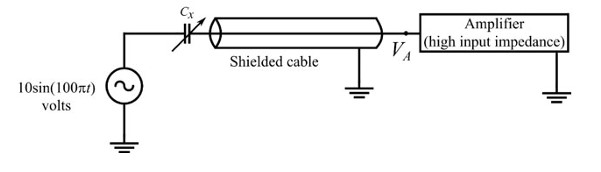
\includegraphics[width=0.7\columnwidth]{figs/q12.jpg}
\caption*{}
\label{fig:q12}
\end{figure}

\hfill{(GATE IN 2020)}

\item Two $100\ohm$ resistors having tolerance $3\%$ and $4\%$ are connected in series. The effective tolerance of the series combination \brak{\text{in \% ,rounded off to one decimal place}} is \rule{2cm}{0.4pt}

\hfill{(GATE IN 2020)}

\item Consider the matrix 
\begin{align*}
M = \myvec{1 & -1 & 0 \\ 1 & -2 & 1 \\ 0 & -1 & 1}.
\end{align*}
 One of the eigenvectors of M is
 
\hfill{(GATE IN 2020)}
\begin{enumerate}
\begin{multicols}{4}
\item
\begin{align*}
\myvec{ -1 \\ 1 \\ 1 }
\end{align*}
\item 
\begin{align*}
\myvec{ 1 \\ 1 \\ -1 }
\end{align*}
\item
\begin{align*}
\myvec{ -1 \\ -1 \\ 1 }
\end{align*}
\item
\begin{align*}
\myvec{ 1 \\ 1 \\ 1 }
\end{align*}
\end{multicols}
\end{enumerate}

\item Consider the differential equation $\frac{dx}{dt} = \sin\brak{x}$, with the initial condition $x\brak{0} = 0$. The solution to this ordinary differential equation is \rule{2cm}{0.4pt}

\hfill{(GATE IN 2020)}
\begin{enumerate}
\begin{multicols}{2}
\item $x\brak{t} = 0$
\item $x\brak{t} = \sin\brak{t}$
\item $x\brak{t} = \cos\brak{t}$
\item $x\brak{t} = \sin\brak{t} - \cos\brak{t}$
\end{multicols}
\end{enumerate}

\item A straight line drawn on an x-y plane intercepts the x-axis at $-0.5$ and the y-axis at $1$. The equation that describes this line is \rule{2cm}{0.4pt}

\hfill{(GATE IN 2020)}
\begin{enumerate}
\begin{multicols}{2}
\item $y = -0.5 x + 1$
\item $y = x - 0.5$
\item $y = 0.5x - 1$
\item $y = 2x + 1$
\end{multicols}
\end{enumerate}

\item The loop transfer function of a negative feedback system is $G\brak{s}H\brak{s} = \frac{1}{s\brak{s-2}}$. The Nyquist plot for the above system \rule{2cm}{0.4pt}

\hfill{(GATE IN 2020)}
\begin{enumerate}
\item encircles $\brak{-1+ j0}$ point once in the clockwise direction
\item encircles $\brak{-1+ j0}$ point once in the counterclockwise direction
\item does not encircle $\brak{-1+j0}$ point
\item encircles $\brak{-1+ j0}$ point twice in the counterclockwise direction
\end{enumerate}

\item $I_1, I_2$ and $I_3$ in the figure below \figref{fig:q13} are mesh currents. The correct 
set of mesh equations for these currents, in matrix form, is \rule{2cm}{0.4pt}
\begin{figure}[H]
\centering
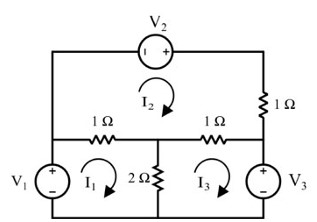
\includegraphics[width=0.5\columnwidth]{figs/q13.jpg}
\caption*{}
\label{fig:q31}
\end{figure}

\hfill{(GATE IN 2020)}



\begin{enumerate}
\begin{multicols}{2}
\item
\begin{align*}
\myvec{ 3 & -1 & -2 \\ -1 & 3 & -1 \\ -2 & -1 & 3 } \myvec{ I_1 \\ I_2 \\ I_3 } = \myvec{ V_1\\ V_2 \\ -V_3 }
\end{align*}
\item
\begin{align*}
\myvec{ 3 & -1 & -2 \\ -1 & 3 & -1 \\ -2 & -1 & -3 } \myvec{ I_1 \\ I_2 \\ I_3 } = \myvec{ V_1 \\ V_2 \\ V_3 }
\end{align*}
\item 
\begin{align*}
\myvec{ -3 & -1 & -2 \\ -1 & 3 & -1 \\ -2 & -1 & 3 } \myvec{ I_1 \\ I_2 \\ I_3 } = \myvec{ V_1 \\ V_2 \\ -V_3 }
\end{align*}
\item 
\begin{align*}
\myvec{ 1 & -1 & -2 \\ -1 & 2 & -1 \\ -2 & -1 & 3 } \myvec{ I_1 \\ I_2 \\ I_3 } = \myvec{ V_1 \\ V_2 \\ V_3 }
\end{align*}
\end{multicols}
\end{enumerate}


\item Consider the function $f\brak{x, y} = x^2 + y^2$. The minimum value the function attains on the line $x + y = 1$ \brak{\text{rounded off to one decimal place}} is \rule{2cm}{0.4pt}

\hfill{(GATE IN 2020)}

\item Consider two identical bags B1 and B2 each containing $10$ balls of identical shapes and sizes. Bag B1 contains $7$ Red and $3$ Green balls, while bag B2 contains $3$ Red and $7$ Green balls. A bag is picked at random and a ball is drawn from it, which was found to be Red. The probability that the Red ball came from bag B1 \brak{\text{rounded off to one decimal place}} is \rule{2cm}{0.4pt}

\hfill{(GATE IN 2020)}

\item The rms value of the phasor current $\underline{I}$ in the circuit shown\figref{fig:q14} \brak{\text{in amperes}} is \rule{2cm}{0.4pt}
\begin{figure}[H]
\centering
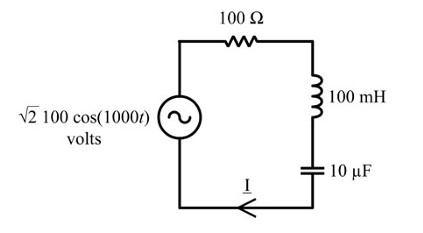
\includegraphics[width=0.4\columnwidth]{figs/q14.jpg}
\caption*{}
\label{fig:q14}
\end{figure}

\hfill{(GATE IN 2020)}

\item In the circuit shown,\figref{fig:q15} the rms value of the voltage across the $100\ohm$ resistor \brak{\text{in volts}} is \rule{2cm}{0.4pt}
\begin{figure}[H]
\centering
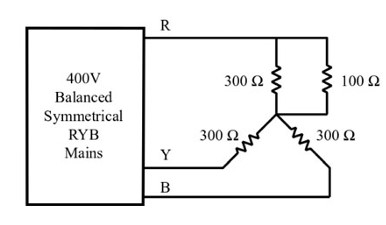
\includegraphics[width=0.4\columnwidth]{figs/q15.jpg}
\caption*{}
\label{fig:q15}
\end{figure}

\hfill{(GATE IN 2020)}

\item Let 
\begin{align*}
g\sbrak{n} = \begin{cases} 1 & n = 0 \\ 0 & n = \pm 1, \pm 2, \pm 3, \dots \end{cases} and h\sbrak{n} = \begin{cases} 1 & n = 0, 3, 6, 9, \dots \\ 0 & \text{otherwise} \end{cases}.
\end{align*}
Consider $y\sbrak{n} = h\sbrak{n} \otimes g\sbrak{n}$, where $\otimes$ denotes the convolution operator. The value of $y\brak{2}$ is \rule{2cm}{0.4pt}

\hfill{(GATE IN 2020)}

\item The loop transfer function of a negative feedback system is given by $G\brak{s}H\brak{s} = \frac{K}{s\brak{s+2}\brak{s+6}}$, where $K > 0$. The value of $K$ at the breakaway point of the root locus for the above system \brak{\text{rounded off to one decimal place}} is \rule{2cm}{0.4pt}

\hfill{(GATE IN 2020)}

\item The system shown\figref{fig:q16} in Fig. \brak{a} has a time response $y\brak{t}$ to an input $r\brak{t} = 10 u\brak{t}$ as shown in Fig. \brak{b}, $u\brak{t}$ being the unit step input. Both $K, \tau$ are positive. The gain $K$ of the system is \rule{2cm}{0.4pt}
\begin{figure}[H]
\centering
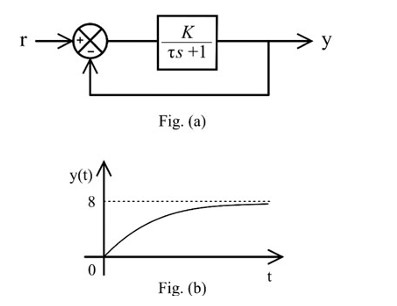
\includegraphics[width=0.8\columnwidth]{figs/q16.jpg}
\caption*{}
\label{fig:q16}
\end{figure}

\hfill{(GATE IN 2020)}

\item Assuming that the opamp used in the circuit shown\figref{fig:q17} is ideal, the reading of the $1$ Hz bandwidth, permanent magnet moving coil \brak{PMMC} type voltmeter \brak{\text{in volts}} is \rule{2cm}{0.4pt}
\begin{figure}[H]
\centering
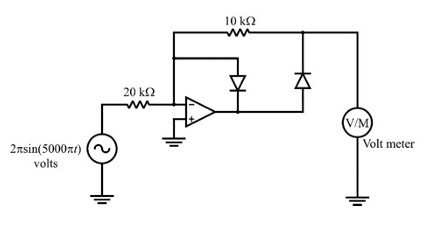
\includegraphics[width=0.6\columnwidth]{figs/q17.jpg}
\caption*{}
\label{fig:q17}
\end{figure}

\hfill{(GATE IN 2020)}

\item If the opamps in the circuit shown\figref{fig:q18} are ideal and $V_x = 0.5$ mV, the steady state value of $V_O$ \brak{\text{in volts, rounded off to two decimal places}} is \rule{2cm}{0.4pt}
\begin{figure}[H]
\centering
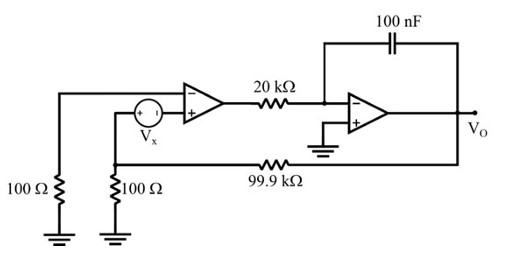
\includegraphics[width=0.6\columnwidth]{figs/q18.jpg}
\caption*{}
\label{fig:q18}
\end{figure}

\hfill{(GATE IN 2020)}

\item Two T-flip flops are interconnected as shown in the figure.\figref{fig:q19} The present state of the flip flops are: $A = 1, B = 1$. The input $x$ is given as $1, 0, 1$ in the next three clock cycles. The decimal equivalent of $\brak{ABy}_2$ with A being the MSB and y being the LSB, after the $3^{rd}$ clock cycle is \rule{2cm}{0.4pt}
\begin{figure}[H]
\centering
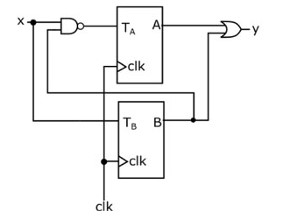
\includegraphics[width=0.5\columnwidth]{figs/q19.jpg}
\caption*{}
\label{fig:q19}
\end{figure}

\hfill{(GATE IN 2020)}

\item The address lines $A_9 \dots A_2$ of a $10$ bit, $1.023$ V full-scale digital to analog converter \brak{DAC} is connected to the data lines $D_7$ to $D_0$ of an 8-bit microprocessor, with $A_1$ and $A_0$ of the DAC grounded. Now, $D_7 \dots D_0$ is changed from $1010~1010$ to $1010~1011$. The corresponding change in the output of the DAC \brak{\text{in mV, rounded off to one decimal place}} is \rule{2cm}{0.4pt}

\hfill{(GATE IN 2020)}

\item The real power drawn by a balanced load connected to a $400$ V, $50$ Hz, balanced, symmetrical 3-phase, 3-wire, RYB sequence mains is measured using the two-wattmeter method. Wattmeter $W_1$ is connected in the R line and wattmeter $W_2$ is connected in the B line. The line current is measured as $\frac{1}{\sqrt{3}}$ A. If the wattmeter $W_1$ reads zero, the reading on $W_2$ \brak{\text{in watts}} is \rule{2cm}{0.4pt}

\hfill{(GATE IN 2020)}

\item A $6\frac{1}{2}$ digit timer-counter is set in the 'time period' mode of operation and the range is set as 'ns'. For an input signal, the timer-counter displays $1000000$. With the same input signal, the timer-counter is changed to 'frequency' mode of operation and the range is set as 'Hz'. The display will show the number \rule{2cm}{0.4pt}

\hfill{(GATE IN 2020)}

\item The circuit shown\figref{fig:q20} uses ideal opamp powered from a supply $V_{CC} = 5$ V. If the charge $q_p$ generated by the piezoelectric sensor is of the form $q_p = 0.1 \sin\brak{10000\pi t}\mu C$, the peak detector output after $10$ cycles of $q_p$ \brak{\text{in volts, rounded off to one decimal place}} is \rule{2cm}{0.4pt}
\begin{figure}[H]
\centering
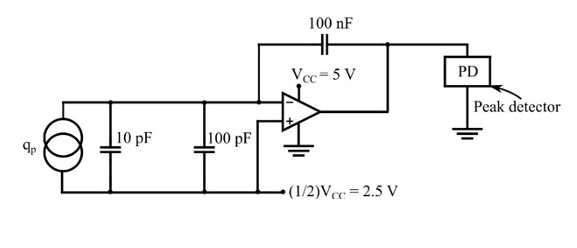
\includegraphics[width=0.6\columnwidth]{figs/q20.jpg}
\caption*{}
\label{fig:q20}
\end{figure}

\hfill{(GATE IN 2020)}

\item A metallic strain gauge of resistance $R_x$ with a gauge factor of $2$ is bonded to a structure made of a metal with modulus of elasticity of $200$ GN/m$^2$. The value of $R_x$ is $1$~k$\ohm$ when no stress is applied. $R_x$ is a part of a quarter bridge with three identical fixed resistors of 1 k$\ohm$ each. The bridge is excited from a DC voltage of $4$ V. The structure is subjected to a stress of $100$ MN/m$^2$. Magnitude of the output of the bridge \brak{\text{in mV, rounded off to two decimal places}} is \rule{2cm}{0.4pt}

\hfill{(GATE IN 2020)}

\item A laser beam of $10$ mm beam diameter is focused onto an optical fibre using a thin biconvex lens as shown in the figure.\figref{fig:q21} The refractive index of the lens is $1.5$. The refractive indices of the core and cladding of the fibre are $1.55$ and $1.54$ respectively. The minimum value of the focal length of the lens to attain the maximum coupling to the fibre \brak{\text{in mm, rounded off to one decimal place}} is \rule{2cm}{0.4pt}
\begin{figure}[H]
\centering
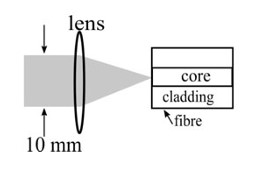
\includegraphics[width=0.4\columnwidth]{figs/q21.jpg}
\caption*{}
\label{fig:q21}
\end{figure}

\hfill{(GATE IN 2020)}

\item As shown in the figure,\figref{fig:q22} a slab of finite thickness $t$ with refractive index $n_2 = 1.5$, has air $\brak{n_1 = 1}$ above and below it. Light of free space wavelength $600$ nm is incident normally from air as shown. For a destructive interference to be observed at R, the minimum value of thickness of the slab $t$ \brak{\text{in nm}} is \rule{2cm}{0.4pt}
\begin{figure}[H]
\centering
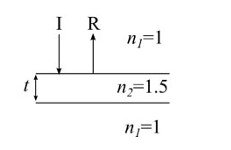
\includegraphics[width=0.3\columnwidth]{figs/q22.jpg}
\caption*{}
\label{fig:q22}
\end{figure}

\hfill{(GATE IN 2020)}

\item Consider the finite sequence $X = \brak{1, 1, 1}$. The Inverse Discrete Fourier Transform \brak{IDFT} of $X$ is given as $\brak{x\brak{0}, x\brak{1}, x\brak{2}}$. The value of $x\brak{2}$ is \rule{2cm}{0.4pt}

\hfill{(GATE IN 2020)}

\item A circuit consisting of capacitors, DC voltage source and an amplifier having a voltage gain $G = -5$ is shown in the figure.\figref{fig:q23} The effective capacitance across the nodes A and B is \rule{2cm}{0.4pt} \brak{\text{in } \mu F, \text{rounded off to one decimal place}}
\begin{figure}[H]
\centering
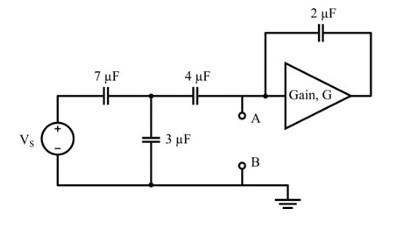
\includegraphics[width=0.5\columnwidth]{figs/q23.jpg}
\caption*{}
\label{fig:q23}
\end{figure}

\hfill{(GATE IN 2020)}

\item Consider the following state variable equations:
\begin{align*}
\dot{x}_1\brak{t} &= x_2\brak{t} \\
\dot{x}_2\brak{t} &= -6x_1\brak{t} - 5x_2\brak{t}
\end{align*}

The initial conditions are $x_1\brak{0} = 0$ and $x_2\brak{0} = 1$. At $t = 1$ second, the value of $x_2\brak{1}$ is \rule{2cm}{0.4pt} \brak{\text{rounded off to two decimal places}} 

\hfill{(GATE IN 2020)}

\item Assume the diodes in the circuit shown\figref{fig:q24} are ideal. The current $I_x$ flowing through the 3 k$\ohm$ resistor \brak{\text{in mA, rounded off to one decimal place}} is \rule{2cm}{0.4pt}
\begin{figure}[H]
\centering
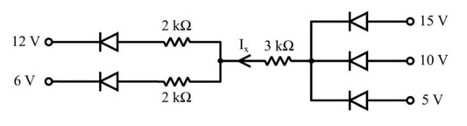
\includegraphics[width=0.6\columnwidth]{figs/q24.jpg}
\caption*{}
\label{fig:q24}
\end{figure}

\hfill{(GATE IN 2020)}

\item A $1000/1$ A, $5$ VA, UPF bar-primary measuring current transformer has $1000$ secondary turns. The current transformer exhibits a ratio error of $-0.1\%$ and a phase error of $3.438$ minutes when the primary current is $1000$ A. At this operating condition, the rms value of the magnetization current of the current transformer \brak{\text{in amperes, rounded off to two decimal places}} is \rule{2cm}{0.4pt}

\hfill{(GATE IN 2020)}

\item The mutual inductances between the primary coil and the secondary coils of a linear variable differential transformer \brak{LVDT} shown in the figure\figref{fig:q25} are $M_1$ and $M_2$. Assume that the self-inductances $L_{s1}$ and $L_{s2}$ remain constant and are independent of $x$. When $x = 0, M_1 = M_2 = M_0$. When $x$ is in the range $\pm 10$ mm, $M_1$ and $M_2$ change linearly with $x$. At $x = +10$ mm or $-10$ mm, the change in the magnitudes of $M_1$ and $M_2$ is $0.25 M_0$. For a particular displacement $x = D$, the voltage across the detector becomes zero when $\abs{V_2} = 1.25\abs{V_1}$. The value of $D$ \brak{\text{in mm, rounded off to one decimal place}} is \rule{2cm}{0.4pt}
\begin{figure}[H]
\centering
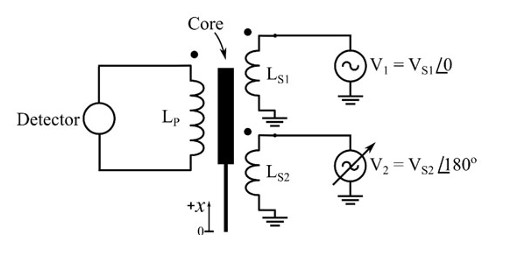
\includegraphics[width=0.5\columnwidth]{figs/q25.jpg}
\caption*{}
\label{fig:q25}
\end{figure}

\hfill{(GATE IN 2020)}

\item In the Maxwell-Wien bridge shown,\figref{fig:q26} the detector D reads zero when $C_1 = 100$ nF and $R_1 = 100$k$\ohm$. The Q factor of the coil is \rule{2cm}{0.4pt}
\begin{figure}[H]
\centering
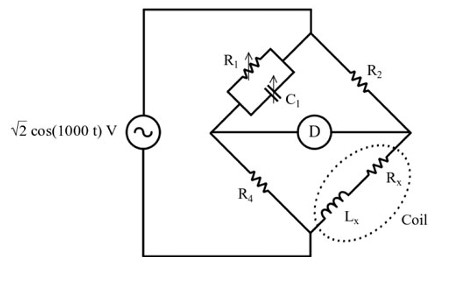
\includegraphics[width=0.5\columnwidth]{figs/q26.jpg}
\caption*{}
\label{fig:q26}
\end{figure}

\hfill{(GATE IN 2020)}

\item The loop transfer function of a negative feedback system is $G\brak{s}H\brak{s} = \frac{2\brak{s+1}}{s^2}$. The phase margin of the system \brak{\text{in degrees, rounded off to one decimal place}} is \rule{2cm}{0.4pt}

\hfill{(GATE IN 2020)}

\end{enumerate}
\end{document}